\documentclass[10pt]{amsart}

\usepackage{algorithm}
\usepackage{algpseudocodex}
\usepackage{amsfonts}
\usepackage{amsmath}
\usepackage{amssymb}
\usepackage{amsthm}
\usepackage[backend=biber, citestyle=numeric-comp, bibstyle=ieee]{biblatex}
\usepackage{changepage}
\usepackage{enumitem}
\usepackage{fancyhdr}
\usepackage{fontspec}
\usepackage{fullpage}
\usepackage[hidelinks]{hyperref}
\usepackage{mathtools}
\usepackage{physics}
\usepackage{thmtools}
\usepackage{tikz}
\usepackage{tikz-3dplot}
\usetikzlibrary{angles, cd, quantikz, quotes, patterns}
\usepackage{titlesec}
\usepackage{wasysym}

\usepackage{tikz-cd}

\usepackage{bookmark}
\usepackage[nameinlink]{cleveref}

\numberwithin{equation}{section}

\titleformat{\section}[runin]{\normalsize\bfseries}{\thesection}{1em}{}[]
\titleformat{\subsection}[runin]{\normalsize\bfseries}{\thesubsection}{1em}{}[]
\titleformat{\subsubsection}[runin]{\normalsize\bfseries}{\thesubsubsection}{1em}{}[]

\addbibresource{finite_abelian_hsp_algorithm_notes.bib}

\theoremstyle{definition}
\newtheorem{theorem}{Theorem}
\newtheorem{definition}{Definition}
\theoremstyle{remark}
\newtheorem{problem}[theorem]{Problem}
\newtheorem{lemma}[theorem]{Lemma}
\newtheorem{remark}[theorem]{Remark}
\newtheorem{observation}[theorem]{Observation}
\newtheorem{example}[theorem]{Example}
\newtheorem{corollary}[theorem]{Corollary}

\renewcommand{\qedsymbol}{\(\blacksquare\)}

\setlength{\parindent}{0pt}

\DeclareMathOperator{\controrot}{CR}
\DeclareMathOperator{\expectation}{E}
\DeclareMathOperator{\gf}{GF}
\DeclareMathOperator{\qft}{QFT}
\DeclareMathOperator{\rk}{rk}
\DeclareMathOperator{\defect}{def}
\DeclareMathOperator{\swapgate}{SWAP}
\DeclareMathOperator{\che}{CHE}
\DeclareMathOperator{\poly}{poly}
\DeclareMathOperator{\Span}{Span}
\DeclareMathOperator{\diag}{diag}

\newcommand{\djk}{\delta_{j, k}}
\newcommand{\tlk}{\tilde{\lambda_k}}

\newcommand{\evalat}[2]{\left.{#1}\middle|\right._{#2}}

% SOURCE: https://tex.stackexchange.com/questions/296151/double-head-and-hook-arrow
\newcommand{\hookdoubleheadrightarrow}{%
  \hookrightarrow\mathrel{\mspace{-15mu}}\rightarrow
}

\newcommand{\draftcomment}[2]{\textcolor{#1}{#2}}

\renewcommand{\algorithmicrequire}{\textbf{Given:}}
\renewcommand{\algorithmicensure}{\textbf{Return:}}

\begin{document}
    valentinpi \hfill Last Change: \today{}

    \section*{Notes on the Finite Abelian HSP Algorithm}

    \section{Introduction} \label{introduction}

    We quickly introduce the necessary notions, facts and the quantum algorithm, with appropriate citations. Recall the finite Abelian Hidden Subgroup Problem (HSP): Given a finite Abelian group \((G, +)\), a subgroup \(H \leq G\) and some \(f\colon G \to X\) with \(X\) an appropriate set, s.t. \(f|_{gH}\) is constant and \(f|_{gH}=f|_{hH} \rightarrow g = h\) for all \(g, h \in G\). Our goal is to find a generator \(\Gamma \subseteq H\) for \(H\) using a quantum algorithm\footnote{Classically, this problem is difficult, as the prime factorization problem shows \cite[p. 24]{Lomont}.}.

    \begin{enumerate}[label=(\roman*)]
        \item Since the left cosets of \(H\) induce a partition of \(G\) \cite[pp. 36-37]{Fischer}, choosing \(X\), s.t. \(|X| \geq |G/H| = |G|/|H|\) \cite[p. 38]{Fischer}, e.g. via \(X \coloneqq \{0, 1\}^{x}\) for some \(x \in \mathbb{N}_{\geq 1}\), \(x \geq \lceil \log_2(|G/H|) \rceil\) suffices.
        \item \label{introduction_1} How do we store group elements in \(G\) in a quantum register? We can do that using qudits, because \(G \cong \bigoplus_{j=1}^{k} \mathbb{Z}_{N_j}\) with \(k \in \mathbb{N}_{\geq 1}\) and \(\{N_1, ..., N_k\} \subseteq \mathbb{N}_{\geq 2}\) \cite[pp. 132-135]{Fischer}, where we take the direct sum of the groups, i.e. the elements of \(G\) can be taken to be tuples \(G \ni g \coloneqq (g_1,...,g_k) \in \prod_{j=1}^k \mathbb{Z}_{N_j}\) \cite[pp. 53-54]{Fischer}. Note that we also call \(N_1, ..., N_k\) \emph{elementary divisors}. We take such a decomposition and appropriate qudits as given here\footnote{Finding such a decomposition is difficult, although a quantum algorithm exists \cite[p. 17]{Lomont}.}.
    \end{enumerate}

    To formulate the quantum algorithm, an analogon for the \(\mathbb{Z}_N\) Quantum Fourier Transform for \(G\) must be defined. This is done via characteristics.

    \section{Characteristics}

    \begin{definition}[{\cite[p. 17]{Lomont}}]
        A \emph{characteristic} over \(G\) is a group homomorphism \((G, +) \to (\mathbb{C}^* \coloneqq \mathbb{C} \setminus \{0\}, \cdot)\).
    \end{definition}
    \begin{lemma}[{\cite[p. 18]{Lomont}}]
        The following statements are true.
        \begin{enumerate}[label=(\roman*)]
            \item The \emph{set of characteristics of \(G\)}, \(\chi(G) \coloneqq \{\chi\colon G \to \mathbb{C}^* \mid \chi \text{ is a characteristic over } G\}\), equipped with the composition of maps, is a group.
            \item The map \(G \hookdoubleheadrightarrow \chi(G), g \mapsto \chi_g\) is a group isomorphism, where we call \(\chi_g\colon G \to \mathbb{C}^*, h \mapsto \prod_{j=1}^k \omega_{N_j}^{g_jh_j}\) the \emph{characteristic induced by \(g\)}.
        \end{enumerate}
    \end{lemma}

    \section{Orthogonal Subgroups}

    \begin{definition}[{\cite[p. 18]{Lomont}}]
        For \(H \subseteq G\) a subgroup of a group \(G\), we define its \emph{orthogonal subgroup} as
        \begin{align}
            H^\perp \coloneqq \{g \in G \mid \chi_g(H) = \{1\}\}
        \end{align}
    \end{definition}

    \begin{lemma}[{\cite*[pp. 19-20]{Lomont}}] \label{orthogonal_subgroups_lemma_1}
        The following statements hold.
        \begin{enumerate}[label=(\roman*)]
            \item \label{orthogonal_subgroups_lemma_1_1} \(H^{\perp} \leq G\)
            \item \label{orthogonal_subgroups_lemma_1_2} \(H^\perp \cong G/H\)
            \item \label{orthogonal_subgroups_lemma_1_3} \(H^{\perp \perp} = H\)
        \end{enumerate}
    \end{lemma}

    Note that we included statement \ref{orthogonal_subgroups_lemma_1_1} here to justify the name in the definition.

    \section{General Fourier Transform}

    \begin{definition}[{\cite[p. 20]{Lomont}}]
        We define the \emph{Quantum Fourier Transform of the Group \(G\)} as
        \begin{align}
            \text{QFT}_G \coloneqq \frac{1}{|G|} \sum_{g, h \in G} \chi_g(h) \ketbra{g}{h} \in \mathbb{C}^{|G| \times |G|}
        \end{align}
    \end{definition}

    For \(G = \mathbb{Z}_N\), \(N \in \mathbb{N}_{\geq 1}\), we thus have \(|G| = N\) and \(\chi_g(h) = e^{i2\pi\frac{g h}{N}}\) for any \(g, h \in G\), meaning that this corresponds to the Quantum Fourier Transform \(\text{QFT}_N\). We further set \(\ket{H'} \coloneqq \frac{1}{|H'|} \sum_{h \in H} \ket{h}\) for any subgroup \(H' \leq G\). Also, we have \(\text{QFT}_G\ket{0} = |G|^{-1/2}\sum_{g \in G} \ket{g}\) by definition.

    \begin{lemma}[{\cite[pp. 19-21, p. 23]{Lomont}}] \label{general_qft_lemma_1}
        The following statements are true.
        \begin{enumerate}[label=(\roman*)]
            \item \(\text{QFT}_G\) is unitary.
            \item \label{general_qft_lemma_1_2} We have \(\text{QFT}_G = \bigotimes_{j=1}^k \text{QFT}_{\mathbb{Z}_{N_j}} = \bigotimes_{j=1}^k \text{QFT}_{N_j}\) for a finite Abelian group \(G\) as in \Cref{introduction}, \ref{introduction_1}.
            \item \label{general_qft_lemma_1_3} \(\text{QFT}_G \ket{H} = \ket{H^\perp}\)
        \end{enumerate}
    \end{lemma}

    Note that in \Cref{general_qft_lemma_1} \ref{general_qft_lemma_1_2}, each quantum fourier transform acts on a single qudit. If we only allow prime qudits, we may use the decomposition of \(G\) into cyclic groups of prime power order \cite[p. 136]{Fischer}. Statement \ref{general_qft_lemma_1_3} of \Cref{general_qft_lemma_1} compactly describes the action of the general fourier group on a subgroup: It flips the group into its orthogonal complement. Applying \(\text{QFT}_G\) then again gives \(\ket{H}\) by \Cref{orthogonal_subgroups_lemma_1} \ref{orthogonal_subgroups_lemma_1_3}.

    \begin{figure}[!hbtp]
        \centering
        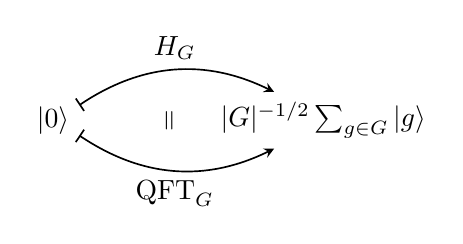
\begin{tikzpicture}[>=stealth, semithick]
            \node (H) at (0, 0) {\(\ket{0}\)};
            \node[right=-1cm] (Hp) at (3, 0) {\(|G|^{-1/2}\textstyle\sum_{g \in G}\ket{g}\)};
            \path[|->] (H) edge[bend left=30] node[above] {\(H_G\)} (Hp);
            \path[|->] (H) edge[bend right=30] node[below] {\(\text{QFT}_G\)} (Hp);
            \node[rotate=90] at (1.5, 0) {\(=\)};
        \end{tikzpicture}
        \hspace{2cm}
        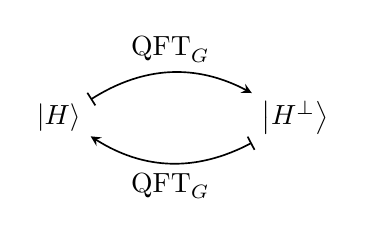
\begin{tikzpicture}[>=stealth, semithick]
            \node (H) at (0, 0) {\(\ket{H}\)};
            \node (Hp) at (3, 0) {\(\ket{H^\perp}\)};
            \path[|->] (H) edge[bend left=30] node[above] {\(\text{QFT}_G\)} (Hp);
            \path[|->] (Hp) edge[bend left=30] node[below] {\(\text{QFT}_G\)} (H);
        \end{tikzpicture}
    \end{figure}

    In the figure, \(H_G\) denotes the Hadamard operator for \(G\), which may be defined by the natural generalization \(\ket{h} \mapsto |G|^{-1/2} \sum_{g \in G} \prod_{j=1}^k(-1)^{g_jh_j} \ket{g}\) for any \(h \in G\). There is one more additional property that is useful.

    \begin{lemma}[{\cite[p. 20-21]{Lomont}}] \label{general_quantum_fourier_transform_commutation_property}
        Setting for any \(t \in G\)
        \begin{align}
            \tau_t \coloneqq \sum_{g \in G} \ketbra{t+g}{g} \text{ and } \phi_t \coloneqq \sum_{g \in G} \chi_g(t)\ketbra{g}{g}
        \end{align}
        to be its associated translation and phase shifting operators, we have the commutation
        \begin{align}
            \text{QFT}_G\tau_t = \phi_t\text{QFT}_G
        \end{align}
    \end{lemma}

    \section{The Quantum Algorithm}

    We now present the full quantum algorithm along with an analysis. The following is due to \cite[pp. 22-23]{Lomont}.

    {\centering\begin{minipage}{\linewidth}
        \vspace{-0.25cm}
        \begin{algorithm}[H]
            \caption{\textsc{Quantum Algorithm for Solving the Finite Abelian HSP}}
            \label{finite_abelian_hsp_quantum_algorithm}
            \begin{algorithmic}[1]
                \Require A finite Abelian group in its cyclic decomposition \(G = \bigoplus_{j=1}^k \mathbb{Z}_{N_j}\) with \(\{N_1, ..., N_k\} \subseteq \mathbb{N}_{\geq 2}\), \(k \in \mathbb{N}_{\geq 1}\), a function \(f\colon G \to X\) hiding a subgroup \(H \leq G\) as described in \Cref{introduction} with \(X \coloneqq \{0, 1\}^x\), \(x \in \mathbb{N}_{\geq 1}\), \(x \geq \lceil\log_2(|G|/|H|)\rceil\), a qudit register \(\ket{\Phi} \coloneqq \ket{0}\ket{0} \in S(\bigotimes_{j=1}^k \mathbb{C}^{N_j} \otimes \mathbb{C}^{|X|})\) and an oracle \(U_f \in \mathbb{C}^{|G||X| \times |G||X|}\) with \(\ket{g}\ket{h} \mapsto \ket{g}\ket{h \oplus f(g)}\) for all \(g \in G, h \in X\).
                \Ensure A generator \(\Gamma \subseteq G\) for \(H\).
                \State \(\ket{\Phi} \gets (\text{QFT}_G^\dagger \otimes E_{|X|}) \ket{\Phi}\) \label{finite_abelian_hsp_quantum_algorithm_1}
                \State \(\ket{\Phi} \gets U_f \ket{\Phi}\)
                \State \(\ket{\Phi} \gets (\text{QFT}_G \otimes E_{|X|}) \ket{\Phi}\)
                \State Measure \(\ket{\Phi}\) wrt. the observable \(\{\Span(\{\ket{g}\ket{h} \mid h \in X\} \mid g \in G)\}\) and obtain an index element \(g \in G\). \label{finite_abelian_hsp_quantum_algorithm_5}
                \State Collect \(1+\log_2(|G|) \eqqcolon t_1\) elements \(g^1, ..., g^{t_1} \in G\) by repeating steps \ref{finite_abelian_hsp_quantum_algorithm_1} to \ref{finite_abelian_hsp_quantum_algorithm_5}.
                \State Form the equation system \(Ah \coloneqq \begin{pmatrix}
                    \alpha_jg_j^i
                \end{pmatrix}_{\substack{1 \leq i \leq t_1\\1 \leq j \leq k}} (h_j)_{1 \leq j \leq k} = 0\) with \(h \in G\) and \(\alpha_j \coloneqq d/N_j\) for any \(j \in \{1, ..., k\}\), where \(d \coloneqq \text{lcm}(\{N_1, ..., N_k\})\). Compute the SNF \(D \in \mathbb{Z}_d^{t_1 \times k}\) of \(A\), and associated unimodular matrices \(U \in \mathbb{Z}_d^{t_1 \times t_1}\) and \(V \in \mathbb{Z}_d^{k \times k}\).
                \State Sample \(1+\log_2(|G|) \eqqcolon t_2\) random solutions \(h^1, ..., h^{t_2}\) to the equation system \(Dh' \equiv 0 \bmod d\) for \(h' \in G\).
                \State \Return \(\{Vh^1, ..., Vh^{t_2}\}\)
            \end{algorithmic}
        \end{algorithm}
    \end{minipage}\par}

    \begin{figure}[!hbtp]
        \centering
        \begin{quantikz}
            \lstick{\(\ket{0}\)} \qw & \gate[wires=1]{\text{QFT}_G^\dagger} \qw & \gate[wires=2]{U_f} \qw & \gate[wires=1]{\text{QFT}_G} \qw & \meter{\(g\)}\\
            \lstick{\(\ket{0}\)} \qw & \qw & \qw
        \end{quantikz}
    \end{figure}

    \phantom{}

    Note that we used the notation \(S(C^n) \coloneqq \{x \in \mathbb{C}^n \mid \norm{x} = 1\}\) for any \(n \in \mathbb{N}\).

    \textbf{Algorithm Analysis of the Quantum Part} Let \(T \subseteq G\) be a transversal wrt. \(G/H\), i.e. a set of representatives of the induced partition. Applying the first steps yields
    \begin{align}
        \ket{0}\ket{0} &\xmapsto{\text{QFT}_G^\dagger \otimes E_{|X|}} \frac{1}{\sqrt{|G|}} \sum_{g \in G}\ket{g}\ket{0}\\
        &\xmapsto{U_f} \frac{1}{\sqrt{|G|}} \sum_{g \in G}\ket{g}\ket{f(g)} = \frac{1}{\sqrt{|T|}} \sum_{t \in T}\ket{t+H}\ket{f(t)} = \frac{1}{\sqrt{|T|}} \sum_{t \in T}\tau_t\ket{H}\ket{f(t)}\\
        &\xmapsto{\text{QFT}_G \otimes E_{|X|}} \frac{1}{\sqrt{|T|}} \sum_{t \in T}\text{QFT}_G\tau_t\ket{H}\ket{f(t)} \overset{\ref{finite_abelian_hsp_quantum_algorithm_analysis_1_1}}{=} \frac{1}{\sqrt{|H^\perp|}} \sum_{t \in T}\phi_t\ket{H^\perp}\ket{f(t)}
    \end{align}

    \begin{enumerate}[label=(\arabic*), wide]
        \item \label{finite_abelian_hsp_quantum_algorithm_analysis_1_1} Use the commutation relation from \Cref{general_quantum_fourier_transform_commutation_property}, apply \Cref{general_qft_lemma_1} \ref{general_qft_lemma_1_3} and then use the fact that \(|T| = |G/H| = |H^\perp|\) by \Cref{orthogonal_subgroups_lemma_1} \ref{orthogonal_subgroups_lemma_1_2}.
    \end{enumerate}

    Note the phase shifting operator \(\phi_t\) for any \(t \in T\) in the resulting state does not influence measurements, so we have successfully, using the general QFT and the oracle, stored a uniform superposition of the elements in \(\ket{H^\perp}\) in the first register. This suggests that we may repeatedly measure on this register to obtain random elements from \(H^\perp\). We will apply the following lemma on random generators.

    \begin{lemma}[{\cite[pp. 76-77]{Lomont}}] \label{randomly_chosen_group_generator_lemma}
        Let \(G\) be a finite group and \(t \in \mathbb{N}\). Then for \(t + \lceil \log_2(|G|) \rceil\) uniformly randomly chosen elements \(g_1, ..., g_{t + \lceil \log_2(|G|) \rceil} \in G\), we have
        \begin{align}
            \Pr(\langle g_1, ..., g_{t + \lceil \log_2(|G|) \rceil} \rangle = G) \geq 1-\frac{1}{2^t}
        \end{align}
    \end{lemma}

    Better results for this exist \cite[p. 77]{Lomont}, but this lemma suffices. However, it is still not clear how to obtain a generator for \(H\).

    \textbf{Obtaining a Generator} Assume for now that we have obtained elements \(g^1, ..., g^\ell \in G\) with some \(\ell \in \mathbb{N}_{\geq 1}\), s.t. \(\langle g^1, ..., g^\ell \rangle = H^\perp\). Since \(H = H^{\perp\perp}\), we have by definition for any \(h \in G\), that \(h \in H\), iff \(\chi_h(g^j) = 1\) for any \(j \in \{1, ..., \ell\}\), as annihilating a generator suffices for the definition of being in the orthogonal complement.

    We first reformulate the solution condition via the orthogonal complement in terms of a linear system by norming the complex roots we consider. Let \(d \coloneqq \text{lcm}(\{N_1, ..., N_k\})\) be the least common multiple of the elementary divisors of \(G\). Fix for now some \(j' \in \{1, ..., \ell\}\). Let \(\alpha_{j'} \coloneqq d/N_{j'}\). Then \(\omega_{N_j} = e^{i 2 \pi / N_j} = \omega_d^{\alpha_{j'}}\). Furthermore, \(\chi_h(g^{j'}) = \prod_{j=1}^k \omega_d^{\alpha_jh_jg_j^{j'}} = 1\), iff \(\sum_{j=1}^k \alpha_j h_j g_j^{j'} \equiv 0 \bmod d\). Letting \(j'\) be loose now, giving the system of congruences
    \begin{align}
        \begin{array}{c}
            \sum_{j=1}^k \alpha_j g_j^1 h_j \equiv 0 \bmod d\\
            \sum_{j=1}^k \alpha_j g_j^2 h_j \equiv 0 \bmod d\\
            \vdots\\
            \sum_{j=1}^k \alpha_j g_j^\ell h_j \equiv 0 \bmod d\\
        \end{array} \label{generator_recovery_soe}
    \end{align}
    or in matrix notation \(\begin{pmatrix}
        \alpha_jg_j^i
    \end{pmatrix}_{\substack{1 \leq i \leq \ell\\1 \leq j \leq k}} (h_j)_{1 \leq j \leq k} = 0 \eqqcolon Ah\) over \(\mathbb{Z}_d\), where we now interpret \(h\) as a column vector. If we are able to obtain enough solutions to this system of congruences, we can generate \(H\) with high probability. The necessary solution technique is the \emph{Smith Normal Form}. Let \(R\) be a principal ideal ring and \(m, n, d \in \mathbb{N}_{\geq 1}\) for the following few definitions and theorems.

    \begin{definition}[{\cite[p. 1069]{Hafner_1991}}]
        We define the following notions.
        \begin{enumerate}[label=(\roman*), wide]
            \item An invertible square matrix \(A \in R^{n \times n}\), \(n \in \mathbb{N}_{\geq 1}\), is called \emph{unimodular}.
            \item Let \(A \in R^{m \times n}\) be some matrix, \(r \coloneqq \text{rk}(A)\) in the associated \(R\)-module and let \(U \in R^{m \times m}\), \(V \in R^{n \times n}\) be unimodular. A matrix \(D \in R^{m \times n}\), s.t.
            \begin{align}
                D = UAV = \begin{pmatrix}
                    s_1\\
                        & \ddots\\
                        &        & s_r\\
                        &        &      & 0\\
                        &        &      &   & \ddots\\
                        &        &      &   &        & 0
                \end{pmatrix}
            \end{align}
            where the omitted entries in either width or height, depending on \(m \leq n\) or \(m > n\), are zero and \(s_i|s_{i+1}\) for any \(i \in \{1, ..., r-1\}\), is called the \emph{Smith Normal Form} (SNF) of \(A\).
        \end{enumerate}
    \end{definition}

    \begin{theorem}[{\cite[pp. 1073-1074]{Hafner_1991}}]
        Any matrix \(A \in \mathbb{Z}^{m \times n}\) admits to a SNF, which can be computed in time \(\tilde{O}(m^3n\log_2(m))\), additionally obtaining the similarity matrices.
    \end{theorem}

    With \(\tilde{O}\), we denote a looser version of the \(O\)-notation, in this case omitting a few logarithmic factors. This is not the best possible result, see e.g. \cite[pp. 273-274]{Storjohann_1996}, but it is one of the simpler algorithms recovering the unimodular similarity matrices as well in the general, thus possibly singular, case.

    \begin{remark}
        In \cite[p. 23]{Lomont}, it is stated that \cite{Storjohann_1996} gives algorithms for computing both the SNF of a matrix over \(\mathbb{Z}\), as well as the equivalence matrices, but the latter is contradicted in \cite[p. 268]{Storjohann_1996}.
    \end{remark}

    Let \(t_1, t_2 \in \mathbb{N}_{\geq 1}\) be loose. We first obtain \(t_1 + \log_2(|G|)\) elements generating \(H^\perp\) with probability \(\geq 1-1/2^{t_1}\). After computing the SNF \(D = UAV\), we have \(U^{-1}DV^{-1}=A\), where we interpret first \(A\) over \(\mathbb{Z}_d\) and then \(\mathbb{Z}\), assuming \(d \in O(1)\) in our runtime considerations. Afterwards, we interpret all matrices over \(\mathbb{Z}_d\) again. We obtain a uniformly random solution to the diagonal inversion problem \(Dh' \equiv 0 \bmod d\) and set \(h \coloneqq Vh'\), yielding \(Ah = U^{-1}DV^{-1}Vh' = 0\). Thus, we may obtain \(t_2 + \log_2(|G|)\) elements of \(H\) this way, which form a generator with probability \(\geq 1 - 1/2^{t_2}\). In total, we obtain a generator of \(H\) with probability \(\geq (1-1/2^{t_1})(1-1/2^{t_2})\). Letting \(t_1 = t_2 = 1\), this is \(\geq 1/4\), which means that we may execute the algorithm four times in expectation.

    \textbf{Runtime Analysis} We apply \(2k \in O(\log_2(N))\) QFT gates and use an oracle call in the first three steps of the algorithm. Note that we assume efficient implementations for the qudit unitaries \(\text{QFT}_{N_1}, ..., \text{QFT}_{N_k}\), as these operations are local. The main cost thus stems from the computation of the SNF. Since \(t_1 \in O(\log_2(|G|))\), we require a runtime of \(\tilde{O}(\log_2^3(|G|)\log_2^{(2)}(|G|))\), where \(\log_2^{(2)} \coloneqq \log_2 \circ \log_2\).

    \begin{theorem}
        \Cref{finite_abelian_hsp_quantum_algorithm} solves the HSP for a finite Abelian group with probability \(\geq 1/4\) in time \(\tilde{O}(\log_2^3(|G|)\log_2^{(2)}(|G|))\).
    \end{theorem}

    \printbibliography{}
\end{document}
